\chapter{Cluster response}

\section{Timing}

\subsection{\gps timestamp, electronics}

When considering coincidences between stations the accuracy of the
timing is crucial. Similar to the offsets between detectors in a
station, offsets between stations have been found. These can be caused
by different detector cable lengths, \gps antennae cable length, and
possibly something in the electronics of the \hisparc box.

Determining the station offset requires many coincidences. The number of
coincidences between stations is inversely correlated to the the
distance between them. Just as the time difference distribution between
detectors the station time difference is dominated by time differences
due to the arrival direction of the showers. This time difference
increases with distance $\Delta t = r * \sin{\theta}$.

\begin{figure}
    \centering
    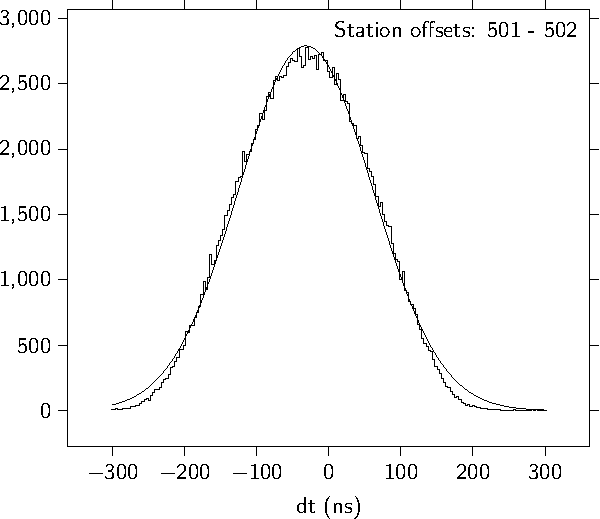
\includegraphics[width=0.6\textwidth]{plots/response/station_offsets_501_502.pdf}
    \caption{\captitle{Coincidence time difference distribution.} The
             time difference between events in coincidence detected by
             station 501 and 502 in the period 2010-2014. The width ..
             due to distance between stations and showers under angles.
             The mean is \SI{-26.6}{\nano\second}.}
    \label{fig:station_offsets_501_502}
\end{figure}

